%priprava posamezne ure
%tukaj zaporedoma napisemo{st. zaporedne ure}{datum}{naslov}{poglavje}{oblika dela}{pripomocki}
\begin{priprava}{}{}{Kombinatorika}{Binomski izrek}{frontalna}{tabla}

\didopomba{Predstavimo Pascalov trikotnik (slika desno) -- kako se ga skonstruira (vsota sosednjih dveh da spodnje število), kar se načeloma pove na začetku 1. letnika pri izrazih. Brez posebnega uvoda. Potem pa narediš še trikotnik s binomskimi simboli (slika levo, ki jo s tremi pikcami nadaljuješ do $ n $-te vrstice) in jih vprašaš, a je to slučaj, da se vrednosti ujemajo? Ne, ker vsota sosednjih dveh da število pod njima po zadnji lastnosti binomskega simbola v prejšnjem poglavju.}

\begin{figure}[h]
    \centering
    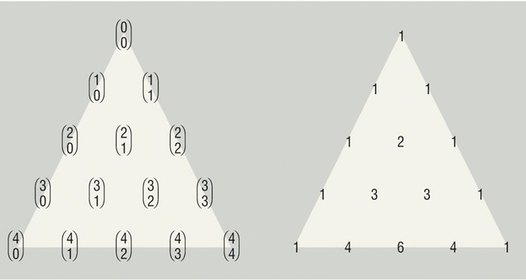
\includegraphics[width=0.8\textwidth]{slike/pascal.jpg}
    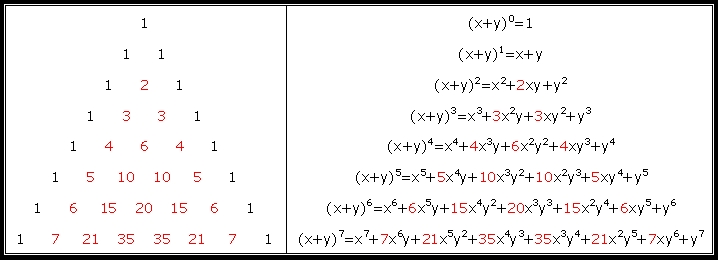
\includegraphics[width=\textwidth]{slike/pascal2.jpg}
\end{figure}

\textbf{Binomki izrek:}

$ (a + b)^n = \binom n 0 a^n + \binom n 1 a^{n-1} b + \binom n 2 a^{n-2} b^2 + \ldots + \binom n r a^{n-r} b^r + \ldots + \binom n {n-1} ab^{n-1} + \binom n n b^n $

$ (a + b)^n = \sum_{r = 0}^n \binom n r a^{n-r} b^r $

\vaje{
Vaje:
\begin{itemize}
    \item Iščemo moč potenčne množice: $ \binom n 0 + \binom n 1 + \binom n 2 + \ldots + \binom n {n-1} + \binom n n = (1 + 1)^n = 2^n $ ( $ a $ in $ b $ sta enaka 1.)
    \item Zapiši 4. člen izraza $ (x \sqrt{x} + x^{-5})^10 $ \didopomba{$ r = 3, a = x \sqrt{x}, b = x^{-5} $}
    \item Poenostavi $ (1 - i)^5 $ ipd.
\end{itemize}
}
    
\end{priprava}